%%%% utfprpgtex-poster.tex, 2018/09/28
%%%% Copyright (C) 2018 Luiz E. M. Lima (luizeduardomlima@gmail.com)
%%
%% Este arquivo pode ser distribuído e/ou modificado sob as condições da
%% Licença Pública do Projeto LaTeX, tanto a versão 1.3 desta licença ou (à sua
%% opção) qualquer versão posterior.
%% A versão mais recente desta licença está disponível em
%%   http://www.latex-project.org/lppl.txt
%% e a versão 1.3 ou posterior faz parte de todas as distribuições de LaTeX
%% versão 2005/12/01 ou posterior.
%%
%% Este arquivo tem o estado de manutenção da LPPL `mantida'.
%%
%% O mantenedor atual deste arquivo é Luiz E. M. Lima.
%%
%% Este projeto consiste dos arquivos utfprpgtex-poster.sty e
%% utfprpgtex-poster.tex.
%%
%% utfprpgtex-poster.tex é o arquivo principal do modelo LaTeX (não oficial)
%% para produção de poster da Universidade Tecnológica Federal do Paraná
%% (UTFPR). Foi desenvolvido baseado na classe beamer, disponível em
%% <http://ctan.org/pkg/beamer/>, e no pacote beamerposter, disponível em
%% <http://ctan.org/pkg/beamerposter/>.

%% Classe e opções de documento
\documentclass[final]{beamer}

%% Passagem de opções para pacotes
\PassOptionsToPackage{english}{babel}%% Suporte multilíngue
\PassOptionsToPackage{%% Utiliza o modo poster da classe beamer --- Opções
  size = custom,%% Tamanho personalizado
  width = 80,%% Largura em centímetros
  height = 200,% Altura em centímetros
  scale = 1.5,%% Escala de fontes
  debug,%% Modo de depuração
}{beamerposter}

%% Pacotes utilizados
\usepackage{utfprpgtex-poster}%% Estilos do modelo

%% Referências
\AtBeginBibliography{\footnotesize}%% Tamanho de fonte
\addbibresource{utfprpgtex-poster.bib}%% Nome de arquivo

%% Informações do documento
\title{%% Título do poster
Flexible LED and Its Applications
}
\subject{Assunto}%% Assunto do poster, e.g.: {Nome do Evento}
\author{%% Autor(es)
  Tingliang ZHANG\inst{1}%
}
\institute{%% Instituição(ões) e e-mail(s)
  \inst{1}\utfprname, Beijing, China%
  \par e-mail: \email[1]{zhangtl16@mails.tsinghua.edu.cn}%
}
\date{}%% Data --- Comente para gerar a data atual

%% Início do documento
\begin{document}

\begin{frame}[t, fragile = singleslide]{}

\begin{columns}[t]%% Cabeçalho

\begin{column}{0.02\textwidth}
\end{column}

\begin{column}{0.18\textwidth}
\flushleft

\includegraphics[width = 0.8\columnwidth]{./Logos/logo-event}%% Logomarca superior-esquerdo
%\vspace*{\baselineskip}
%
\includegraphics[width = 0.8\columnwidth]{./Logos/logo-org}%% Logomarca inferior-esquerdo
\end{column}

\begin{column}{0.6\textwidth}
\titlepage
\end{column}

\begin{column}{0.18\textwidth}
\flushright

\includegraphics[width = 0.8\columnwidth]{./Logos/logo-tsinghua}%% Logomarca superior-direito
%\vspace*{\baselineskip}
%
\includegraphics[width = 0.8\columnwidth]{./Logos/logo-inst-ext}%% Logomarca inferior-direito
\end{column}

\begin{column}{0.02\textwidth}
\end{column}

\end{columns}

\begin{columns}[t]

\begin{column}{0.45\textwidth}

\begin{block}{INTRODUCTION}
This project proposes a reliable flexible LED production solution, and proposes several flexible LED application scenarios, which are expected to drive LED production capacity and promote the development of emerging industries such as LED fashion and lighting show.

Domestic flexible LED technology is still in its infancy. This project proposes a reliable flexible LED production solution and proposes a new form of artistic expression.

The initial flexible LED solution is intended to use Adafruit LED Sequins and LILYPAD, which are connected by copper wires wrapped in braided wires. The pads are specially treated to make them difficult to fall off under harsh environments such as machine wash, and the whole system is dispersed so that it can be embedded. Among the fabrics. At the same time try new materials, such as conductive thermoplastics, to further improve reliability and open up new forms of artistic expression.

It will be divided into the following application scenarios for development: (not limited to the application scenarios presented below)

Application Scenario 1: Interactive RGB-LED dot matrix wearable device for EEG control 

By detecting the EEG signal, the user's mood is displayed in a flexible LED array on a wearable device such as a casual hat in the form of Emoji, thereby achieving the purpose of interaction.

At the same time, the patterns on the wearable device can be customized as a modern form of self-expression. Similar additional features can be implemented with other modules, such as heart rate + breathing + body temperature detection.

Since the flexible circuit is washable and reliable, it can be directly cleaned using a washing machine, and the unburdened user experience is achieved. Compared with other embedded wearable devices, the advantages of consumers are higher.

Related technology:
The TGAM EEG module can process and output brainwave frequency spectra, EEG signal quality, original brainwaves and three Neurosky eSense parameters: concentration, relaxation and blink detection. Due to its low energy consumption and a simple dry contact point with the human body interface, it can be adapted for use in flexible wearable devices.

Application Scenario 2: Flexible LED Panel for the Photography Industry

At present, the photographic mats commonly used in the photography industry are often made by tiling LED strips on flexible materials, with low reliability and low cost, and a single color tone. If the flexible LED is used to make the lighting panel, not only the reliability is greatly improved, but also the good performance of the flexible LED can realize more applications, such as making a spherical light source of the Gonit.

In addition, for individual users of diy photography creation, single color source and illumination mode photography fill light is difficult to meet the demand. Flexible led lighting facilities can achieve a personalized custom effect of the fill light source.


  The main innovations of this project are:
  \begin{itemize}
    \item porting traditional PCB circuits to flexible substrates;
    \item facilitates the production of personalized custom wearable devices;
    \item uses the brain-computer interface to develop Emoji controls.
  \end{itemize}
\end{block}

\end{column}

\begin{column}{0.45\textwidth}

\begin{block}{Component selection}
Compared to the WS2812 Breakout board, the LilyPad Pixel's LEDs are located within a purple ring. This approach makes it easy to stitch into clothing or other textiles, so it can be easily embedded in our smart textile projects.

FLORA is Adafruit's miniaturized development platform for wearable devices that can be connected to a computer via a USB interface for direct programming, and it also supports USB HID. FLORA is not the first Arduino development platform for wearable devices. Leah Buechley designed and manufactured a LilyPad in 2007, but FLORA's flash and SRAM are twice as large as LilyPad, and FLORA is smaller than LilyPad. 

The TGAM module includes a TGAT chip, which is a highly integrated single-chip EEG sensor that can output three Neurosky eSense parameters, can perform analog-to-digital conversion, detect abnormal conditions of poor contact, and filter out eye-electric noise and 50/ 60hz AC interference.

This TGAM module can process and output brainwave frequency spectrum, EEG signal quality, original brainwaves and three Neurosky eSense parameters: concentration, relaxation and blink detection. The interface with the human body requires only a simple dry contact point, so it can be easily used in toys, video games and health equipment, and because of low energy consumption, it is suitable for use in battery-powered portable consumer products.
\end{block}

%\end{column}

%\begin{column}{0.45\textwidth}

\begin{block}{Manufacturing process}
The wire is directly selected from the 0.04mm diameter straight-welded QA-1-130 enameled wire. The room temperature resistance is less than 10 ohm/meter, the bendability is very good, and the surface has an insulating layer to prevent short circuit caused by the two wires crossing during weaving. The strength and elongation factor are also fully compliant with the project requirements.

Later, it may be possible to use some advanced new materials, such as wires for conductive fabrics: https://patents.google.com/patent/CN104674573A/zh.

The components use fabric-friendly pads like FLORA and LilyPad Pixel: pads that are wide and flush with the component plane. This also increases the robustness while ensuring flexibility (favorable for sewing on clothing or other textiles). (The contact area between the pad and the wire is large)

The splitter board uses a plate PCB similar to a multi-rotor hub/electrical switchboard/plant protection drone splitter board, because there are only one or two splitter boards in the whole circuit, and the board surface is extremely small. Does not affect the overall wear experience of the fabric.

Integration of the overall circuit with the fabric/clothing

First, we will discuss the routing: Due to the robustness of the circuit, we will sew a very thin enameled wire (similar to twisted pair) into the fabric with a sewing machine, because the WS2813 used in the project is used in the project. The two-in and two-out series structure, so for the convenience of wiring, the two-two connection lines are similar to the twisted pair sewing process. Individually required three-wire/four-wire parallel (such as VCC and GND leads) is implemented using a four-color sewing machine. If a single wire condition cannot be avoided, use two equivalent enameled wires instead of a single wire connection.

Secondly, the discussion of LilyPad Pixel placement of single-layer tulle and double-layer translucent fabric:


\begin{itemize}
\item For double-layer translucent fabrics, we place the LilyPad Pixel between two layers of fabric so that the pad joints are protected to the utmost in everyday life and in the washing machine.

\item The single-layer tulle is different. We place the LilyPad Pixel on one side of the fabric. The side of the LilyPad Pixel is used on the outside. Due to the fixing effect of the four "woven" enameled wires, the daily use will not fall off, but it is used. Washing machines should be cautious.
\end{itemize}

In mass production, the textile machine can be customized to achieve high reliability and automatic production. This work only shows the feasibility of this sewing process.
\end{block}

\end{column}

\end{columns}

\begin{columns}[t]

\begin{column}{0.945\textwidth}

\begin{block}{RESULT}
We have connected and debugged the above circuits and are currently working on integrating the circuits into the fabric. As Figuras~\ref{fig:graficoxy1} shows.

\begin{figure}[!htb]
\centering
\caption{Exemple of Flexible LED.}
\label{fig:graficoxy1}
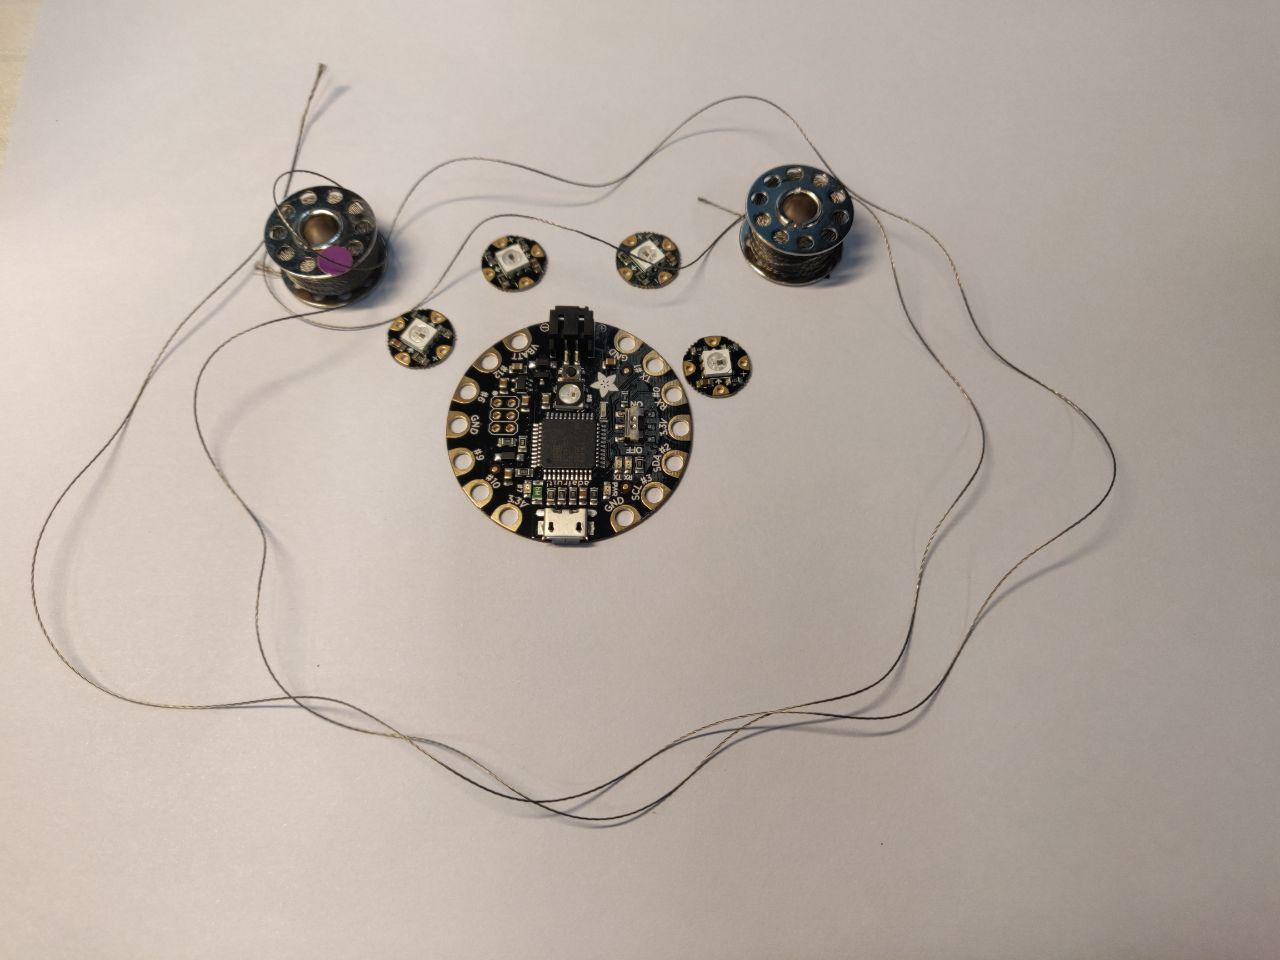
\includegraphics[width = 0.25\columnwidth]{./Figuras/LED.jpg}
\end{figure}

\end{block}

\end{column}

\end{columns}

\begin{columns}[t]

\begin{column}{0.45\textwidth}

\begin{block}{CONCLUSIONS}
The universal application of smart wearable devices in the future will promote the development of flexible embedded circuits. The flexible circuit process proposed in this paper will show its value in the near future.
\end{block}

\end{column}

\begin{column}{0.45\textwidth}

\begin{block}{Acknowledgements}
\footnotesize
I would like to express my special thanks of gratitude to SPARK 12 as well as our university who gave me the golden opportunity to do this wonderful project, which also helped me in doing a lot of Research and i came to know about so many new things I am really thankful to them.
\vfill

\includegraphics[height = 90mm]{./Logos/logo-event.png}
\hspace*{15mm}

\includegraphics[height = 90mm]{./Logos/logo-tsinghua.jpg}

\end{block}

\end{column}

\end{columns}

\begin{columns}[t]

\begin{column}{0.945\textwidth}
\vfill

\end{column}

\end{columns}

\end{frame}

%% Fim do documento
\end{document}
